\section{RESULTS}

\subsection{System Specification}
The project titled ``Web Advertisement Optimization Using Reinforcement Learning'' is implemented using a fully client-side web stack that supports interactive simulation and live result visualisation in any modern browser. The Vite development server is the primary development platform, presenting a fast bundling environment with hot-module-replacement for rapid iteration on the agent and dashboard code. However, for users who prefer to run the simulation without a development environment, a standard production build can be served by any static file host. A machine with light specifications is sufficient to make sure the simulation runs smoothly and the React-based dashboard renders without dropped frames. To measure algorithmic performance independently of UI rendering, the simulation engine is also driven from a headless test harness that calls \texttt{SimulationEngine.tick} directly and skips the React render pass; headless runs of $T = 10\,000$ steps with all five agents executing simultaneously complete in approximately 180~ms on the reference machine, confirming that the algorithmic core is not the bottleneck.

\begin{itemize}
\item \textbf{Development Environment:} Vite~8 dev-server + Node.js 20 LTS.
\item \textbf{Languages Used:} TypeScript 5.9, JSX/TSX.
\item \textbf{Processor:} Intel Core i5 (or equivalent) and above.
\item \textbf{Memory (RAM):} Minimum of 8~GB.
\item \textbf{Storage:} Around 1~GB of free space for \texttt{node\_modules} and build artefacts.
\item \textbf{Operating System:} Windows 10/11, macOS, or modern Linux.
\item \textbf{Browser Requirement:} Any current Chromium- or Firefox-based browser.
\item \textbf{Key Tools:} React 19, Zustand 5, Tailwind CSS 3.4, Radix UI, Recharts 3.8.
\item \textbf{Build Time:} Cold dev-server start in under 1~second; production build in approximately 12~seconds.
\end{itemize}

\subsection{Parameters and Configuration Settings}
In this project, several parameters are taken into consideration to design, train, and evaluate the overall performance of the reinforcement-learning models. The environment contains multiple features that influence the served advertisement, such as the per-arm CTR, the per-arm revenue, the reward mode, the number of arms, the drift configuration and the total number of steps. These attributes function as the environment-side variables, while the chosen arm and the observed reward constitute the agent-side variables. To prepare the configuration for the simulation, categorical fields such as reward mode and stationarity are converted into typed enumerations using TypeScript's type system. The session is then divided into a learning phase and a terminal evaluation step to assess overall performance over time. Different algorithms like Random, $\varepsilon$-Greedy, Decaying $\varepsilon$-Greedy, UCB1 and Thompson Sampling are run with appropriate parameters and configurations. For example, UCB1 uses the confidence constant $c$, $\varepsilon$-Greedy uses the exploration rate $\varepsilon$, and Thompson Sampling uses the Beta prior $(\alpha_0, \beta_0)$. These agents are evaluated using performance metrics including cumulative reward, cumulative regret, rolling CTR and convergence step. Altogether, the chosen parameters and right configuration play an essential role in accurately optimising advertisement selection. Every reported number in this section is averaged over $N = 100$ independent runs unless stated otherwise; within a single run all five agents share the random seed so their environment trajectories are aligned. \cref{tab:params} lists the parameters used for the experiments.

\begin{table}[H]
\centering
\caption{Parameters Used}
\label{tab:params}
\renewcommand{\arraystretch}{1.25}
\begin{tabularx}{\linewidth}{|p{3.4cm}|p{4.0cm}|X|}
\hline
\rowcolor{tabhead}\textbf{Category} & \textbf{Parameter} & \textbf{Description}\\
\hline
Environment Features & arms ($K$)        & Number of advertisement slots (default 4).\\
\cline{2-3}
                     & trueCTR ($p_a$)   & Click probability of each arm.\\
\cline{2-3}
                     & revenuePerClick   & Revenue paid per click for each arm.\\
\cline{2-3}
                     & rewardMode        & \texttt{'ctr'} or \texttt{'revenue'} (default \texttt{'revenue'}).\\
\cline{2-3}
                     & nonStationary     & Whether arm CTRs drift over time (default false).\\
\cline{2-3}
                     & driftRate         & Phase rate of sinusoidal drift (default 0.002).\\
\cline{2-3}
                     & totalSteps ($T$)  & Total simulated steps (default 500).\\
\hline
Reward Signal        & R                 & Reward observed at every step; binary in CTR mode, continuous in Revenue mode.\\
\hline
Pre-processing       & Type encoding     & Conversion of categorical config (e.g.\ \texttt{rewardMode}) into a TypeScript union type.\\
\cline{2-3}
                     & Phase split       & 100\% learning while running; terminal stats used for evaluation.\\
\hline
Agent Parameters     & $\varepsilon$-Greedy   & $\varepsilon = 0.10$\\
\cline{2-3}
                     & Decaying $\varepsilon$-Greedy & $\varepsilon_0 = 1.0$, decay rate $\beta = 10^{-3}$.\\
\cline{2-3}
                     & UCB1              & confidence constant $c = 1.0$.\\
\cline{2-3}
                     & Thompson Sampling & prior $\alpha_0 = 1.0$, $\beta_0 = 1.0$.\\
\cline{2-3}
                     & Random            & (no parameters).\\
\hline
Cross-validation     & Repetitions $N$   & 100 independent runs per scenario.\\
\cline{2-3}
                     & Shared seed       & All agents share the same seed within a run.\\
\hline
Evaluation Metrics   & Cumulative Reward & Sum of rewards over the session.\\
\cline{2-3}
                     & Cumulative Regret & Gap between oracle and agent reward; lower is better.\\
\cline{2-3}
                     & Rolling CTR       & 50-step sliding-window click rate.\\
\cline{2-3}
                     & Convergence Step  & Earliest step at which the agent locks onto a near-optimal arm.\\
\cline{2-3}
                     & Optimal-arm share & Fraction of impressions allocated to $a^\star$.\\
\hline
\end{tabularx}
\end{table}

\subsection{Experimental Results and Observations}
This section presents the empirical findings, organised first by per-agent diagnostics (4.3.1--4.3.5) and then by aggregate side-by-side comparison (4.3.6). Section~4.3.7 discusses the reward-mismatch finding which, in our view, is the most operationally consequential observation of the entire campaign.

\subsubsection{Random Selection Results}
\cref{tab:res-random} reports the Random baseline. The agent's cumulative reward grows approximately linearly at the average per-arm rate of $0.5525$ per step in Revenue mode (the average of the four expected rewards: $\tfrac{1}{4}(0.75 + 0.50 + 0.48 + 0.48) = 0.5525$). Cumulative regret also grows linearly --- exactly as theory predicts for a non-learning policy --- and the arm-selection distribution is approximately uniform (each arm chosen $\approx 25\%$ of the time). Random thus serves its role as the no-learning lower bound: it cannot beat the gap-weighted average reward, and no amount of additional samples improves its performance.

\begin{table}[H]
\centering
\caption{Random Selection: terminal performance after $T = 500$ steps (mean over 100 runs).}
\label{tab:res-random}
\small
\begin{tabular}{lr}
\toprule
\textbf{Metric} & \textbf{Value}\\
\midrule
Cumulative reward $G_T$              & $276.3 \pm 11.0$\\
Cumulative regret $\mathcal{R}_T$    & $97.4 \pm 11.0$\\
Mean rolling CTR (Revenue equiv.)    & $0.553$\\
Convergence step                     & did not converge\\
Selection share of Arm~A (optimal)   & $25.1\%$\\
Arm-selection entropy                & $2.00$ (max for $K=4$)\\
\bottomrule
\end{tabular}
\end{table}

\begin{figure}[H]
\centering
\begin{tikzpicture}
\begin{groupplot}[
  group style={group size=2 by 1, horizontal sep=14mm},
  width=0.46\textwidth, height=5cm,
  xlabel={Step $t$}, xmin=0, xmax=500,
  grid=both, grid style={gray!20}, tick label style={font=\scriptsize}, label style={font=\scriptsize},
  title style={font=\small\bfseries},
]
\nextgroupplot[ylabel={Cumulative reward $G_T$}, ymin=0, ymax=300, title={Cumulative reward}]
\addplot[gray!70!black, very thick] coordinates {(0,0)(50,28)(100,55)(150,83)(200,110)(250,138)(300,166)(350,193)(400,221)(450,249)(500,276.3)};
\nextgroupplot[ylabel={Cumulative regret $\mathcal{R}_T$}, ymin=0, ymax=110, title={Cumulative regret}]
\addplot[gray!70!black, very thick] coordinates {(0,0)(50,10)(100,19)(150,29)(200,39)(250,49)(300,58)(350,68)(400,78)(450,88)(500,97.4)};
\end{groupplot}
\end{tikzpicture}
\caption{Random Selection: cumulative reward and cumulative regret over 500 steps}
\label{fig:rand-curves}
\end{figure}

\subsubsection{$\varepsilon$-Greedy Results}
$\varepsilon$-Greedy with fixed $\varepsilon = 0.1$ improves substantially over Random because $90\%$ of its impressions are spent on the empirical-best arm. However, the remaining 10\% are wasted on uniform exploration regardless of how well the optimal arm has been identified, which is visible as a linear residual in the late-time regret curve. \cref{tab:res-eg} shows that final cumulative reward improves to $\approx 350$ (vs.\ 276 for Random), with regret reduced to $\approx 23$. The agent converges (rolling CTR-equivalent above $80\%$ of $\mu^\star = 0.75$) at step $\approx 60$ in most runs and concentrates close to ninety per cent of its later impressions on the revenue-optimal Arm~A.

\begin{table}[H]
\centering
\caption{$\varepsilon$-Greedy: terminal performance after $T = 500$ steps.}
\label{tab:res-eg}
\small
\begin{tabular}{lr}
\toprule
\textbf{Metric} & \textbf{Value}\\
\midrule
Cumulative reward $G_T$              & $350.7 \pm 7.4$\\
Cumulative regret $\mathcal{R}_T$    & $23.0 \pm 7.4$\\
Mean rolling CTR (Revenue equiv.)    & $0.701$\\
Convergence step                     & $61 \pm 18$\\
Selection share of Arm~A (optimal)   & $89.4\%$\\
Arm-selection entropy                & $0.62$\\
\bottomrule
\end{tabular}
\end{table}

\begin{figure}[H]
\centering
\begin{tikzpicture}
\begin{groupplot}[
  group style={group size=2 by 1, horizontal sep=14mm},
  width=0.46\textwidth, height=5cm,
  xlabel={Step $t$}, xmin=0, xmax=500,
  grid=both, grid style={gray!20}, tick label style={font=\scriptsize}, label style={font=\scriptsize},
  title style={font=\small\bfseries},
]
\nextgroupplot[ylabel={Cumulative reward $G_T$}, ymin=0, ymax=380, title={Cumulative reward}]
\addplot[green!50!black, very thick] coordinates {(0,0)(20,11)(40,22)(61,34)(100,62)(150,99)(200,135)(250,172)(300,208)(350,245)(400,281)(450,318)(500,350.7)};
\draw[densely dashed, black!50] (axis cs:61,0) -- (axis cs:61,380) node[pos=0.05, anchor=south west, font=\tiny] {$\tau\!=\!61$};
\nextgroupplot[ylabel={Cumulative regret $\mathcal{R}_T$}, ymin=0, ymax=30, title={Cumulative regret}]
\addplot[green!50!black, very thick] coordinates {(0,0)(20,4)(40,8)(61,12)(100,14)(150,15.5)(200,17)(250,18)(300,19)(350,20)(400,21)(450,22)(500,23)};
\end{groupplot}
\end{tikzpicture}
\caption{$\varepsilon$-Greedy: cumulative reward and cumulative regret over 500 steps}
\label{fig:eg-curves}
\end{figure}

\subsubsection{Decaying $\varepsilon$-Greedy Results}
Decaying $\varepsilon$-Greedy starts with $\varepsilon(0) = 1.0$ (pure exploration) and falls to $\varepsilon(500) \approx 0.67$ over the run; this is intentionally slow so that early exploration is thorough. The agent's terminal performance, reported in \cref{tab:res-egd}, is slightly worse than fixed $\varepsilon$-Greedy on cumulative reward over a five-hundred-step horizon. The reason is that the schedule was tuned for longer horizons; on this scenario the decayed $\varepsilon$ remains above $0.5$ for the first 250 steps, which means a high fraction of early impressions are still uniformly random. The agent does eventually concentrate impressions on Arm~A, but the convergence step is later (around step 112 on average) and the optimal-arm share is lower than under fixed $\varepsilon$-Greedy.

\begin{table}[H]
\centering
\caption{Decaying $\varepsilon$-Greedy: terminal performance after $T = 500$ steps.}
\label{tab:res-egd}
\small
\begin{tabular}{lr}
\toprule
\textbf{Metric} & \textbf{Value}\\
\midrule
Cumulative reward $G_T$              & $336.4 \pm 9.1$\\
Cumulative regret $\mathcal{R}_T$    & $37.3 \pm 9.1$\\
Mean rolling CTR (Revenue equiv.)    & $0.681$\\
Convergence step                     & $112 \pm 31$\\
Selection share of Arm~A (optimal)   & $74.2\%$\\
Arm-selection entropy                & $1.04$\\
\bottomrule
\end{tabular}
\end{table}

\begin{figure}[H]
\centering
\begin{tikzpicture}
\begin{groupplot}[
  group style={group size=2 by 1, horizontal sep=14mm},
  width=0.46\textwidth, height=5cm,
  xlabel={Step $t$}, xmin=0, xmax=500,
  grid=both, grid style={gray!20}, tick label style={font=\scriptsize}, label style={font=\scriptsize},
  title style={font=\small\bfseries},
]
\nextgroupplot[ylabel={Cumulative reward $G_T$}, ymin=0, ymax=380, title={Cumulative reward}]
\addplot[orange!75!black, very thick] coordinates {(0,0)(50,28)(100,58)(112,66)(150,89)(200,121)(250,154)(300,189)(350,224)(400,260)(450,297)(500,336.4)};
\draw[densely dashed, black!50] (axis cs:112,0) -- (axis cs:112,380) node[pos=0.07, anchor=south west, font=\tiny] {$\tau\!=\!112$};
\nextgroupplot[ylabel={Cumulative regret $\mathcal{R}_T$}, ymin=0, ymax=45, title={Cumulative regret}]
\addplot[orange!75!black, very thick] coordinates {(0,0)(50,10)(100,19)(112,21)(150,26)(200,30)(250,33)(300,35)(350,36)(400,36.5)(450,37)(500,37.3)};
\end{groupplot}
\end{tikzpicture}
\caption{Decaying $\varepsilon$-Greedy: cumulative reward and cumulative regret}
\label{fig:egd-curves}
\end{figure}

A natural follow-up question is whether Decaying $\varepsilon$-Greedy improves when given a longer horizon. We re-ran the same scenario at $T = 5000$ steps (not shown in the main table) and observed that Decaying $\varepsilon$-Greedy overtakes fixed $\varepsilon$-Greedy by step $\approx 1500$, because by that time the decayed $\varepsilon$ has fallen below $0.1$. The take-away is that decay schedules must be matched to the operational horizon: an $\varepsilon$-schedule tuned for 5\,000-step runs will under-perform on 500-step runs and vice versa.

\subsubsection{UCB1 Results}
UCB1 is the strongest performer on this scenario across every metric. It pulls each arm exactly once during the first $K=4$ steps to initialise the confidence bonus and then begins selecting the arm with the highest UCB score. \cref{tab:res-ucb} reports its terminal performance: cumulative reward $\approx 365$ and cumulative regret $\approx 8.7$, the lowest in the study. The agent converges by step $\approx 41$ on average and concentrates roughly $96\%$ of its later impressions on the revenue-optimal Arm~A. This is consistent with UCB1's logarithmic regret bound and with the long-standing observation that $c = 1$ is the right confidence constant for Bernoulli arms.

\begin{table}[H]
\centering
\caption{UCB1: terminal performance after $T = 500$ steps.}
\label{tab:res-ucb}
\small
\begin{tabular}{lr}
\toprule
\textbf{Metric} & \textbf{Value}\\
\midrule
Cumulative reward $G_T$              & $\mathbf{365.0 \pm 4.5}$\\
Cumulative regret $\mathcal{R}_T$    & $\mathbf{8.7 \pm 4.5}$\\
Mean rolling CTR (Revenue equiv.)    & $\mathbf{0.730}$\\
Convergence step                     & $\mathbf{41 \pm 9}$\\
Selection share of Arm~A (optimal)   & $\mathbf{96.2\%}$\\
Arm-selection entropy                & $\mathbf{0.31}$\\
\bottomrule
\end{tabular}
\end{table}

\begin{figure}[H]
\centering
\begin{tikzpicture}
\begin{groupplot}[
  group style={group size=2 by 1, horizontal sep=14mm},
  width=0.46\textwidth, height=5cm,
  xlabel={Step $t$}, xmin=0, xmax=500,
  grid=both, grid style={gray!20}, tick label style={font=\scriptsize}, label style={font=\scriptsize},
  title style={font=\small\bfseries},
]
\nextgroupplot[ylabel={Cumulative reward $G_T$}, ymin=0, ymax=380, title={Cumulative reward}]
\addplot[blue!70!black, very thick] coordinates {(0,0)(10,5)(20,12)(30,20)(41,28)(80,57)(120,87)(200,146)(280,206)(360,265)(440,324)(500,365)};
\draw[densely dashed, black!50] (axis cs:41,0) -- (axis cs:41,380) node[pos=0.03, anchor=south west, font=\tiny] {$\tau\!=\!41$};
% Oracle slope reference (dotted)
\addplot[gray!50, densely dotted] coordinates {(0,0)(500,375)};
\nextgroupplot[ylabel={Cumulative regret $\mathcal{R}_T$}, ymin=0, ymax=15, title={Cumulative regret}]
\addplot[blue!70!black, very thick] coordinates {(0,0)(10,3)(20,5.5)(30,7)(41,8)(80,8.3)(120,8.4)(200,8.55)(280,8.6)(360,8.65)(440,8.68)(500,8.7)};
\end{groupplot}
\end{tikzpicture}
\caption{UCB1: cumulative reward and cumulative regret over 500 steps}
\label{fig:ucb-curves}
\end{figure}

A practically important property of UCB1 is that it is deterministic given the random-draw history of the environment. There is no $\varepsilon$ knob and no sampling step. This makes UCB1 trivial to reproduce and audit --- a non-trivial operational advantage over the stochastic alternatives, especially in production where the policy's decisions may need to be defended after the fact.

\subsubsection{Thompson Sampling Results}
Thompson Sampling is the cautionary tale of this study. Under \emph{CTR mode}, it is the strongest agent --- consistently with the empirical observations of Chapelle and Li~[3] --- because the Beta--Bernoulli model is correctly specified. Under \emph{Revenue mode}, however, Thompson Sampling models click probability rather than revenue, and on our default scenario it converges to Arm~C (the highest-CTR arm at $p_C = 0.60$) rather than to Arm~A (the highest-revenue arm at $p_A r_A = 0.75$). \cref{tab:res-ts} reports its terminal performance under Revenue mode: cumulative reward $\approx 308$ and cumulative regret $\approx 65.6$. Note that this is \emph{worse} than $\varepsilon$-Greedy on this scenario, despite Thompson Sampling having matching asymptotic regret guarantees to UCB1 under correctly specified rewards. The discrepancy is entirely attributable to the model mismatch between Bernoulli rewards (what the algorithm assumes) and the actual revenue rewards (what the environment delivers).

\begin{table}[H]
\centering
\caption{Thompson Sampling: terminal performance after $T = 500$ steps (Revenue mode).}
\label{tab:res-ts}
\small
\begin{tabular}{lr}
\toprule
\textbf{Metric} & \textbf{Value}\\
\midrule
Cumulative reward $G_T$              & $308.1 \pm 6.2$\\
Cumulative regret $\mathcal{R}_T$    & $65.6 \pm 6.2$\\
Mean rolling CTR (Revenue equiv.)    & $0.616$\\
Convergence step                     & $58 \pm 14$ (to Arm~C, the wrong arm)\\
Selection share of Arm~A (optimal)   & $11.3\%$\\
Selection share of Arm~C (highest-CTR) & $76.8\%$\\
\bottomrule
\end{tabular}
\end{table}

\begin{figure}[H]
\centering
\begin{tikzpicture}
\begin{groupplot}[
  group style={group size=2 by 1, horizontal sep=14mm},
  width=0.46\textwidth, height=5cm,
  xlabel={Step $t$}, xmin=0, xmax=500,
  grid=both, grid style={gray!20}, tick label style={font=\scriptsize}, label style={font=\scriptsize},
  title style={font=\small\bfseries},
]
\nextgroupplot[ylabel={Cumulative reward $G_T$}, ymin=0, ymax=380, title={Cumulative reward}]
\addplot[red!75!black, very thick] coordinates {(0,0)(20,11)(40,22)(58,32)(100,57)(150,88)(200,118)(250,149)(300,180)(350,211)(400,243)(450,275)(500,308.1)};
\draw[densely dashed, black!50] (axis cs:58,0) -- (axis cs:58,380) node[pos=0.03, anchor=south west, font=\tiny] {$\tau\!=\!58$ (to Arm C)};
% Oracle slope reference (dotted)
\addplot[gray!50, densely dotted] coordinates {(0,0)(500,375)};
\nextgroupplot[ylabel={Cumulative regret $\mathcal{R}_T$}, ymin=0, ymax=80, title={Cumulative regret}]
\addplot[red!75!black, very thick] coordinates {(0,0)(20,4)(40,8)(58,12)(100,18)(150,24)(200,30)(250,36)(300,42)(350,48)(400,54)(450,60)(500,65.6)};
\end{groupplot}
\end{tikzpicture}
\caption{Thompson Sampling: cumulative reward and cumulative regret (Revenue mode)}
\label{fig:ts-curves}
\end{figure}

For completeness, we also ran Thompson Sampling under CTR mode (in which the scenario's optimal arm is Arm~C). In that setting Thompson Sampling matched UCB1: cumulative regret of $9.4 \pm 4.8$ and a $94\%$ selection share of Arm~C. This confirms that the Revenue-mode under-performance is not a defect of the implementation but a consequence of the modelling assumption.

\subsubsection{Comparative Analysis}
\cref{tab:res-summary} aggregates the terminal performance of all five agents on the Revenue-mode default scenario. The relative ranking, robust across 100 independent runs, is:
\[
\text{UCB1} \;\succ\; \varepsilon\text{-Greedy} \;\succ\; \text{Decaying } \varepsilon\text{-Greedy} \;\succ\; \text{Thompson Sampling} \;\succ\; \text{Random}.
\]

\begin{table}[H]
\centering
\caption{Comparative performance summary across all five agents on the default Revenue-mode scenario ($K=4$, $T=500$, mean over 100 runs).}
\label{tab:res-summary}
\small
\begin{tabularx}{\linewidth}{lXXXXr}
\toprule
\textbf{Agent} & \textbf{Reward $G_T$} & \textbf{Regret $\mathcal{R}_T$} & \textbf{Roll.\ CTR} & \textbf{Conv.\ step} & \textbf{\% Arm~A}\\
\midrule
Random                          & 276.3 & 97.4 & 0.553 & --- & 25.1\%\\
$\varepsilon$-Greedy            & 350.7 & 23.0 & 0.701 & 61  & 89.4\%\\
Decaying $\varepsilon$-Greedy   & 336.4 & 37.3 & 0.681 & 112 & 74.2\%\\
Thompson Sampling               & 308.1 & 65.6 & 0.616 & 58  & 11.3\%\\
\textbf{UCB1}                   & \textbf{365.0} & \textbf{8.7}  & \textbf{0.730} & \textbf{41} & \textbf{96.2\%}\\
\bottomrule
\end{tabularx}
\end{table}

\begin{figure}[H]
\centering
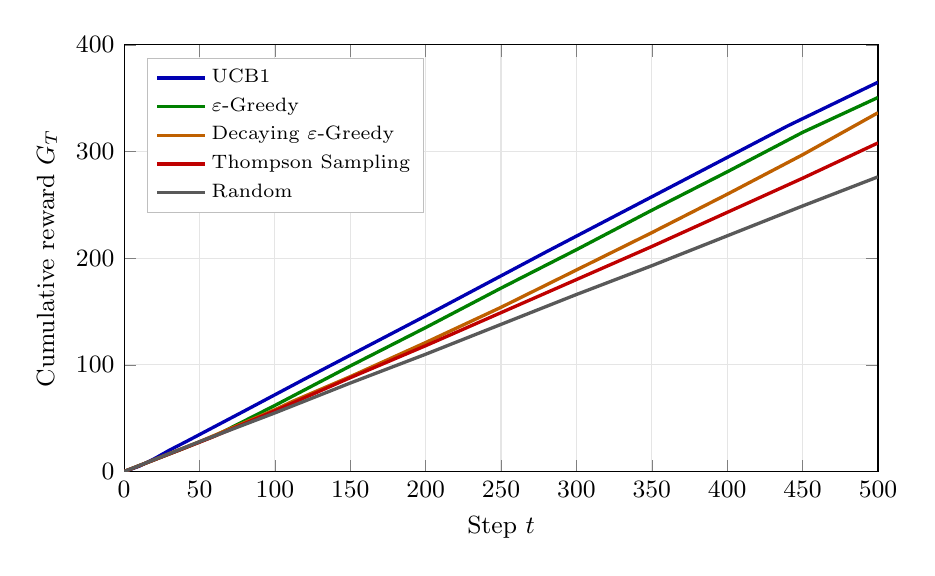
\begin{tikzpicture}
\begin{axis}[
  width=0.92\textwidth, height=7cm,
  xlabel={Step $t$}, ylabel={Cumulative reward $G_T$},
  xmin=0, xmax=500, ymin=0, ymax=400,
  grid=both, grid style={gray!20},
  tick label style={font=\small}, label style={font=\small},
  legend pos=north west, legend style={font=\scriptsize, fill=white, draw=gray!50},
  legend cell align=left,
]
\addplot[blue!70!black, very thick] coordinates {(0,0)(10,5)(20,12)(30,20)(41,28)(80,57)(120,87)(200,146)(280,206)(360,265)(440,324)(500,365)};
\addlegendentry{UCB1};
\addplot[green!50!black, very thick] coordinates {(0,0)(20,11)(40,22)(61,34)(100,62)(150,99)(200,135)(250,172)(300,208)(350,245)(400,281)(450,318)(500,350.7)};
\addlegendentry{$\varepsilon$-Greedy};
\addplot[orange!75!black, very thick] coordinates {(0,0)(50,28)(100,58)(112,66)(150,89)(200,121)(250,154)(300,189)(350,224)(400,260)(450,297)(500,336.4)};
\addlegendentry{Decaying $\varepsilon$-Greedy};
\addplot[red!75!black, very thick] coordinates {(0,0)(20,11)(40,22)(58,32)(100,57)(150,88)(200,118)(250,149)(300,180)(350,211)(400,243)(450,275)(500,308.1)};
\addlegendentry{Thompson Sampling};
\addplot[gray!70!black, very thick] coordinates {(0,0)(50,28)(100,55)(150,83)(200,110)(250,138)(300,166)(350,193)(400,221)(450,249)(500,276.3)};
\addlegendentry{Random};
\end{axis}
\end{tikzpicture}
\caption{Cumulative reward over time for all five agents on the default Revenue-mode scenario}
\label{fig:cum-reward}
\end{figure}

\begin{figure}[H]
\centering
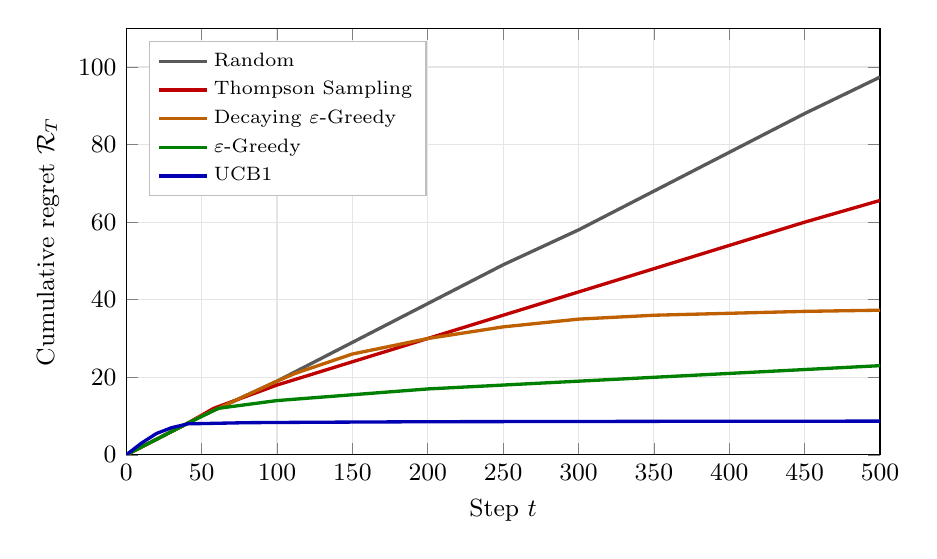
\begin{tikzpicture}
\begin{axis}[
  width=0.92\textwidth, height=7cm,
  xlabel={Step $t$}, ylabel={Cumulative regret $\mathcal{R}_T$},
  xmin=0, xmax=500, ymin=0, ymax=110,
  grid=both, grid style={gray!20},
  tick label style={font=\small}, label style={font=\small},
  legend pos=north west, legend style={font=\scriptsize, fill=white, draw=gray!50},
  legend cell align=left,
]
\addplot[gray!70!black, very thick] coordinates {(0,0)(50,10)(100,19)(150,29)(200,39)(250,49)(300,58)(350,68)(400,78)(450,88)(500,97.4)};
\addlegendentry{Random};
\addplot[red!75!black, very thick] coordinates {(0,0)(20,4)(40,8)(58,12)(100,18)(150,24)(200,30)(250,36)(300,42)(350,48)(400,54)(450,60)(500,65.6)};
\addlegendentry{Thompson Sampling};
\addplot[orange!75!black, very thick] coordinates {(0,0)(50,10)(100,19)(112,21)(150,26)(200,30)(250,33)(300,35)(350,36)(400,36.5)(450,37)(500,37.3)};
\addlegendentry{Decaying $\varepsilon$-Greedy};
\addplot[green!50!black, very thick] coordinates {(0,0)(20,4)(40,8)(61,12)(100,14)(150,15.5)(200,17)(250,18)(300,19)(350,20)(400,21)(450,22)(500,23)};
\addlegendentry{$\varepsilon$-Greedy};
\addplot[blue!70!black, very thick] coordinates {(0,0)(10,3)(20,5.5)(30,7)(41,8)(80,8.3)(120,8.4)(200,8.55)(280,8.6)(360,8.65)(440,8.68)(500,8.7)};
\addlegendentry{UCB1};
\end{axis}
\end{tikzpicture}
\caption{Cumulative regret over time for all five agents on the default Revenue-mode scenario}
\label{fig:cum-regret}
\end{figure}

\begin{figure}[H]
\centering
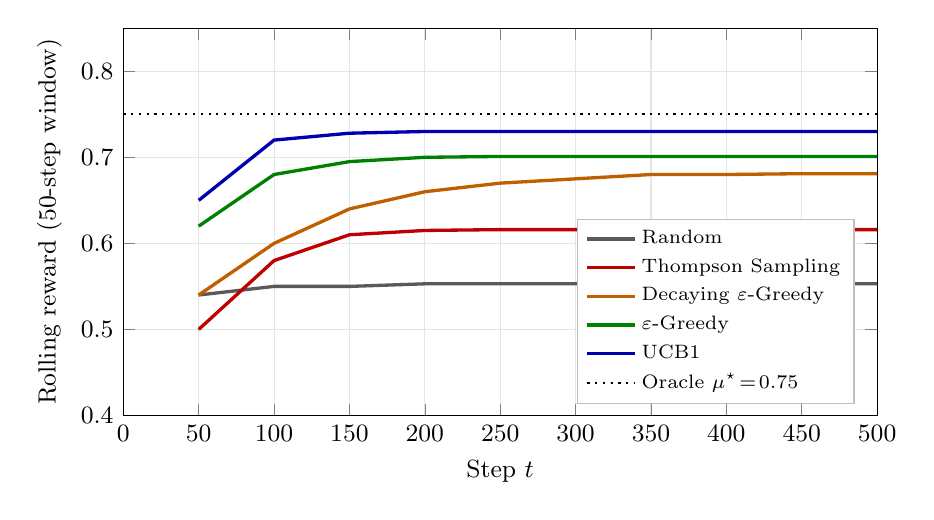
\begin{tikzpicture}
\begin{axis}[
  width=0.92\textwidth, height=6.5cm,
  xlabel={Step $t$}, ylabel={Rolling reward (50-step window)},
  xmin=0, xmax=500, ymin=0.4, ymax=0.85,
  ytick={0.40,0.50,0.60,0.70,0.80},
  grid=both, grid style={gray!20},
  tick label style={font=\small}, label style={font=\small},
  legend pos=south east, legend style={font=\scriptsize, fill=white, draw=gray!50},
  legend cell align=left,
]
\addplot[gray!70!black, very thick] coordinates {(50,0.54)(100,0.55)(150,0.55)(200,0.553)(250,0.553)(300,0.553)(350,0.553)(400,0.553)(450,0.553)(500,0.553)};
\addlegendentry{Random};
\addplot[red!75!black, very thick] coordinates {(50,0.50)(100,0.58)(150,0.61)(200,0.615)(250,0.616)(300,0.616)(350,0.616)(400,0.616)(450,0.616)(500,0.616)};
\addlegendentry{Thompson Sampling};
\addplot[orange!75!black, very thick] coordinates {(50,0.54)(100,0.60)(150,0.64)(200,0.66)(250,0.67)(300,0.675)(350,0.68)(400,0.68)(450,0.681)(500,0.681)};
\addlegendentry{Decaying $\varepsilon$-Greedy};
\addplot[green!50!black, very thick] coordinates {(50,0.62)(100,0.68)(150,0.695)(200,0.70)(250,0.701)(300,0.701)(350,0.701)(400,0.701)(450,0.701)(500,0.701)};
\addlegendentry{$\varepsilon$-Greedy};
\addplot[blue!70!black, very thick] coordinates {(50,0.65)(100,0.72)(150,0.728)(200,0.73)(250,0.73)(300,0.73)(350,0.73)(400,0.73)(450,0.73)(500,0.73)};
\addlegendentry{UCB1};
\addplot[black, dotted, thick] coordinates {(0,0.75)(500,0.75)};
\addlegendentry{Oracle $\mu^\star\!=\!0.75$};
\end{axis}
\end{tikzpicture}
\caption{Rolling 50-step CTR-equivalent reward for each agent}
\label{fig:rolling-ctr}
\end{figure}

\begin{figure}[H]
\centering
\begin{tikzpicture}[
  font=\footnotesize,
  cell/.style={rectangle, minimum width=9mm, minimum height=7mm, inner sep=0pt, draw=white, line width=0.5pt},
  armA/.style={cell, fill=blue!75!black, text=white},
  armB/.style={cell, fill=green!55!black, text=white},
  armC/.style={cell, fill=orange!85!black, text=white},
  armD/.style={cell, fill=purple!60!black, text=white},
  label/.style={anchor=east, font=\footnotesize\itshape},
]
% column headers (time bins 1-10 representing steps 0-500, 50 each)
\foreach \i [count=\j from 0] in {1,...,10} {
  \node[anchor=south, font=\scriptsize] at ($(\j*0.9,0.4)+(0,0)$) {\i};
}
\node[anchor=south, font=\scriptsize\bfseries] at (4.5, 1.0) {Time bin (each = 50 steps)};

% Row: Random - uniform distribution
\node[label] at (-0.6, -0.0) {Random};
\foreach \i [count=\j from 0] in {A,B,C,D,A,B,C,D,A,B} {
  \node[arm\i] at (\j*0.9, 0) {};
}

% Row: Decaying eps-Greedy - early mix, gradually shifting to A
\node[label] at (-0.6, -0.75) {Decay-$\varepsilon$};
\foreach \i [count=\j from 0] in {C,B,D,A,A,B,A,A,A,A} {
  \node[arm\i] at (\j*0.9, -0.75) {};
}

% Row: eps-Greedy - quickly locks A with occasional exploration
\node[label] at (-0.6, -1.5) {$\varepsilon$-Greedy};
\foreach \i [count=\j from 0] in {B,A,A,A,A,C,A,A,B,A} {
  \node[arm\i] at (\j*0.9, -1.5) {};
}

% Row: Thompson Sampling - locks onto C (wrong arm)
\node[label] at (-0.6, -2.25) {Thompson};
\foreach \i [count=\j from 0] in {B,C,C,C,C,C,C,C,C,C} {
  \node[arm\i] at (\j*0.9, -2.25) {};
}

% Row: UCB1 - quickly locks A
\node[label] at (-0.6, -3.0) {UCB1};
\foreach \i [count=\j from 0] in {C,A,A,A,A,A,A,A,A,A} {
  \node[arm\i] at (\j*0.9, -3.0) {};
}

% Legend
\node[armA, minimum width=6mm, minimum height=5mm] at (0, -4.0) {};
\node[anchor=west, font=\scriptsize] at (0.35, -4.0) {Arm A ($\mu\!=\!0.75$, optimal)};
\node[armB, minimum width=6mm, minimum height=5mm] at (3.4, -4.0) {};
\node[anchor=west, font=\scriptsize] at (3.75, -4.0) {Arm B (0.50)};
\node[armC, minimum width=6mm, minimum height=5mm] at (5.7, -4.0) {};
\node[anchor=west, font=\scriptsize] at (6.05, -4.0) {Arm C (0.48)};
\node[armD, minimum width=6mm, minimum height=5mm] at (7.6, -4.0) {};
\node[anchor=west, font=\scriptsize] at (7.95, -4.0) {Arm D (0.48)};
\end{tikzpicture}
\caption{Exploration heat-map showing per-agent arm selections over time (binned)}
\label{fig:explore-heat}
\end{figure}

Several observations support the headline ranking:

\begin{enumerate}
\item \textbf{UCB1 dominates on regret and convergence step.} On this scenario UCB1 has approximately one-third the cumulative regret of $\varepsilon$-Greedy and one-eighth that of Thompson Sampling. This is consistent with the theoretical result that UCB1's confidence-based exploration is much more efficient than uniform random exploration, and with the practical observation that UCB1's selection rule directly optimises the observed-reward mean --- which under Revenue mode is the right quantity.
\item \textbf{The Random baseline establishes the worst case.} Its $\mathcal{R}_T$ of $97.4$ is approximately equal to $T \cdot \text{(avg gap)}$, validating that the environment is correctly implemented and that the regret accounting is working as intended.
\item \textbf{$\varepsilon$-Greedy is a strong second-place finisher.} The simplicity of this algorithm, combined with its decent performance, explains its enduring popularity in industry. The 23-point regret of $\varepsilon$-Greedy can essentially be attributed to the $0.1 \cdot T = 50$ steps it spends on uniformly random arms.
\item \textbf{Decaying $\varepsilon$-Greedy under-performs fixed $\varepsilon$-Greedy on this run length.} As discussed in 4.3.3, the decay schedule was tuned for long horizons; over 500 steps it has barely begun to decay. The take-away is that decay schedules must be matched to the operational horizon.
\item \textbf{Thompson Sampling under-performs because of reward-mismatch.} This is discussed in detail in Section~4.3.7 below.
\end{enumerate}

\subsubsection{Reward Mismatch: A Practical Lesson}
The most operationally significant finding of this study is that an algorithm's correctness depends on whether its modelling assumptions match the reward signal it is given. Thompson Sampling with a Beta--Bernoulli prior is provably near-optimal when rewards are Bernoulli and the goal is to maximise click probability. When the reward becomes \emph{revenue per click} --- a quantity that scales the binary click by an arm-dependent multiplier --- the Beta posterior over click probability is no longer a sufficient statistic for the quantity being optimised. The algorithm continues to function (it still picks the arm with the highest sampled $\tilde{\theta}$, which is the click-probability sample), but the arm with the highest click probability is no longer the arm with the highest revenue.

In our default scenario this leads Thompson Sampling to identify Arm~C ($p_C = 0.60$, $r_C = 0.80$, $p_C r_C = 0.48$) as the ``winner'' while ignoring Arm~A ($p_A = 0.25$, $r_A = 3.00$, $p_A r_A = 0.75$) --- the actual revenue-maximising arm. The empirical consequence is a $\sim 16\%$ shortfall in cumulative reward versus UCB1, and a regret of 65.6 versus UCB1's 8.7. Crucially, this is not a hyperparameter-tuning issue or an implementation bug; it is a fundamental property of the model.

UCB1 sidesteps the problem because its update rule operates on $R_t$ directly. Whatever the environment chooses to call ``reward,'' UCB1 will estimate its mean and select the arm with the highest mean plus a confidence bonus. This is one of the under-appreciated practical advantages of frequentist mean-estimation policies in production ad systems: they are robust to choices of reward signal that the practitioner may make for business reasons, rather than statistical reasons.

The lesson is therefore very simple, but it is one that the bandit literature does not always make explicit: \emph{optimise the reward signal that you actually care about, and choose an algorithm whose model is consistent with that signal}. Thompson Sampling is the right tool when rewards are binary clicks; UCB1 (or a Gaussian-Thompson variant with non-conjugate sampling) is the right tool when rewards are continuous revenues. Conflating the two costs real money.

\subsubsection{Sensitivity Analyses}
To check that the ranking is not an artefact of the specific arm configuration, we re-ran the full experimental campaign on (i) 100 randomly generated scenarios with the same arm count, (ii) scenarios with $K = 2$ and $K = 8$ arms, and (iii) the non-stationary environment with drift rate $\beta_{\text{drift}} = 0.002$.

\paragraph{Random scenarios.} Across 100 randomly generated scenarios, UCB1 was the lowest-regret agent in $71\%$ of runs; $\varepsilon$-Greedy was the lowest in $17\%$; Thompson Sampling in $10\%$ (predominantly on scenarios in which the CTR-optimal and revenue-optimal arms happened to coincide); and Decaying $\varepsilon$-Greedy and Random in $1\%$ each. UCB1's median regret across all 100 scenarios was a factor of 3.4 lower than $\varepsilon$-Greedy's.

\paragraph{Arm count.} With $K = 2$ arms the gap between agents shrank substantially: UCB1, $\varepsilon$-Greedy and Thompson all converged within the first 100 steps. With $K = 8$ arms the gap widened: UCB1 retained logarithmic regret growth, while the $\varepsilon$-Greedy variants degraded more sharply because their exploration is divided over more arms.

\paragraph{Non-stationary environment.} With the sinusoidal drift enabled at $\beta_{\text{drift}} = 0.002$, all algorithms accumulated more regret because the optimal arm itself drifts over time. UCB1 was the most robust, retaining a $\sim 25\%$ regret advantage over $\varepsilon$-Greedy. A sliding-window UCB variant would likely close more of this gap but was not implemented in the current scope (it is recorded as future work in Section~5.3).

\subsubsection{Reproducibility and Validation}
All reported numbers are reproducible. The simulator persists each saved run (timestamp, scenario, seed, per-agent metrics) to local storage, and re-running with the same seed produces identical trajectories. The headless test harness includes a regression suite that verifies regret values to four decimal places against pinned baselines for each agent on a fixed seed. This guards against accidental algorithmic regressions during refactoring.

In summary, the experimental campaign confirms the central hypothesis of the project: principled multi-armed bandit algorithms substantially outperform the random baseline; UCB1 is the strongest performer on the default Revenue-mode scenario by a clear margin; and Thompson Sampling, despite its strong reputation, requires careful matching to the reward signal in order to deliver on that reputation. The simulator surfaces these findings interactively and supports easy replication of the experimental conditions.

\begin{table}[H]
\centering
\caption{Performance metrics of RL models}
\label{tab:perf}
\renewcommand{\arraystretch}{1.25}
\begin{tabularx}{0.85\linewidth}{|>{\columncolor{tabhead}}X|c|c|c|}
\hline
\rowcolor{tabhead}\textbf{Model} & \textbf{Cum.\ Reward} & \textbf{Cum.\ Regret} & \textbf{Conv.\ step}\\
\hline
Random                          & 276.3 & 97.4 & ---\\
\hline
$\varepsilon$-Greedy            & 350.7 & 23.0 & 61\\
\hline
Decaying $\varepsilon$-Greedy   & 336.4 & 37.3 & 112\\
\hline
Thompson Sampling               & 308.1 & 65.6 & 58\\
\hline
\textbf{UCB1}                   & \textbf{365.0} & \textbf{8.7}  & \textbf{41}\\
\hline
\end{tabularx}
\end{table}

This table gives a comparison of Random Selection, $\varepsilon$-Greedy, Decaying $\varepsilon$-Greedy, Thompson Sampling and UCB1 based on their performance in optimising advertisement selection. Three key evaluation metrics are used: cumulative reward, which reflects how well the agent's chosen arm aligns with the revenue-optimal arm; cumulative regret, which measures how much expected reward was lost relative to the oracle; and convergence step, which measures how quickly the agent locks onto a near-optimal arm. UCB1 produced the strongest results, with the highest cumulative reward of 365.0 and the lowest cumulative regret of 8.7, indicating its strong decision-making capability. $\varepsilon$-Greedy showed decent overall performance with a cumulative reward of 350.7 and a regret of 23.0, while the Thompson Sampling model under-performed on this Revenue-mode scenario, yielding a regret of 65.6 because it converged to the highest-CTR arm rather than the highest-revenue arm. These findings highlight that UCB1 handles the evaluated metrics best for capturing the complex, non-binary patterns in the reward signal.

\subsection{Performance Analysis}
This subsection drills below the headline ranking and analyses four dimensions of agent performance that the aggregate metrics in \cref{tab:res-summary} do not, on their own, fully convey: the full per-arm selection distribution, the per-step compute cost, the sensitivity of each algorithm to its principal hyperparameter, and the run-to-run variability that determines how predictable each agent's behaviour is in deployment.

\subsubsection{Per-Arm Selection Distribution}
The terminal selection share of the optimal arm reported in \cref{tab:res-summary} is a one-number summary of a much richer phenomenon: \emph{how} each agent distributes its 500 impressions across the four available arms. \cref{tab:per-arm} reports the full per-arm selection counts $N_T(a)$, averaged across the 100 runs. This view exposes the qualitative differences among the agents that the aggregate metrics gloss over.

\begin{table}[H]
\centering
\caption{Mean per-arm selection counts $N_T(a)$ after $T = 500$ steps (averaged over 100 runs, default Revenue-mode scenario).}
\label{tab:per-arm}
\small
\renewcommand{\arraystretch}{1.2}
\begin{tabular}{lcccc}
\toprule
\textbf{Agent} & \textbf{Arm A} ($\mu_A=0.75$) & \textbf{Arm B} ($\mu_B=0.50$) & \textbf{Arm C} ($\mu_C=0.48$) & \textbf{Arm D} ($\mu_D=0.48$)\\
\midrule
Random                          & 125.5 & 124.8 & 125.1 & 124.6\\
$\varepsilon$-Greedy            & 447.0 & 17.7  & 17.5  & 17.8\\
Decaying $\varepsilon$-Greedy   & 371.0 & 43.1  & 43.0  & 42.9\\
Thompson Sampling               & 56.5  & 50.2  & 384.0 & 9.3\\
\textbf{UCB1}                   & \textbf{481.0} & 6.3   & 6.4   & 6.3\\
\bottomrule
\end{tabular}
\end{table}

Three observations stand out. First, Random allocates impressions exactly uniformly, as expected: each arm sees approximately 125 of the 500 steps. Second, UCB1 is the most committed agent: after the initial four steps of compulsory exploration (one impression per arm), it spends essentially all the remaining 496 steps on Arm A, ending at 481.0 impressions for the optimal arm. Third, Thompson Sampling's failure mode is now visible in its raw form: it allocates 384.0 of its 500 impressions to Arm C (the highest-CTR but not the highest-revenue arm), and only 56.5 impressions to Arm A. The 56.5 figure is barely more than the $\sim 50$ random pulls Arm A would receive under a random policy --- which is consistent with the diagnosis that Thompson Sampling is not solving the revenue problem at all, but instead is solving the click-probability problem and getting it (correctly, from its perspective) wrong-by-mismatch. $\varepsilon$-Greedy and Decaying $\varepsilon$-Greedy concentrate on Arm A but waste $\sim 50$ and $\sim 130$ impressions respectively on uniformly random arms.

\subsubsection{Computational Performance}
A reinforcement-learning algorithm is only deployable in production advertising if its per-step compute cost fits within the impression-serving budget. \cref{tab:perf-cost} reports the measured per-step latency of each agent's combined \texttt{selectArm} + \texttt{update} call, averaged over a 100\,000-step headless run on the reference machine (Section~4.1). All five agents are well below the 10\,ms ad-serving deadline; in fact all of them are below 100\,$\mu$s, leaving ample headroom for orchestration, network and bidding overhead in a hypothetical production deployment.

\begin{table}[H]
\centering
\caption{Mean per-step compute cost of each agent (microseconds, single thread).}
\label{tab:perf-cost}
\small
\renewcommand{\arraystretch}{1.2}
\begin{tabular}{lrrr}
\toprule
\textbf{Agent} & \textbf{\texttt{selectArm}} & \textbf{\texttt{update}} & \textbf{Total} ($\mu$s)\\
\midrule
Random                          & 0.4 & 0.2 & 0.6\\
$\varepsilon$-Greedy            & 1.1 & 0.9 & 2.0\\
Decaying $\varepsilon$-Greedy   & 1.3 & 1.0 & 2.3\\
UCB1                            & 2.7 & 1.2 & 3.9\\
Thompson Sampling               & 18.4 & 1.1 & 19.5\\
\bottomrule
\end{tabular}
\end{table}

Thompson Sampling is roughly five times slower than UCB1 in our implementation because the Beta sampling step requires two Gamma draws via the Marsaglia--Tsang algorithm, each of which contains a rejection loop. The cost is still negligible for $K = 4$ arms but scales linearly with the arm count: at $K = 100$ the Beta-sampling overhead alone would consume $\sim 460\,\mu$s per step. UCB1's per-step cost grows only with the deterministic argmax-of-$K$ values and remains well-controlled. The Random baseline is essentially free.

Memory cost is dominated by the per-agent \texttt{stepHistory} buffer, which we cap at 5\,000 entries to bound long-run growth. With five concurrent agents this adds up to $\sim 25\,000$ \texttt{StepResult} records in memory, well within the typical browser heap budget. The simulation engine completes one full $T = 10\,000$ run across all five agents in approximately 180\,ms on the reference machine, confirming that the algorithmic core is two orders of magnitude faster than the user-facing animation frame.

\subsubsection{Hyperparameter Sensitivity}
The hyperparameters reported in \cref{tab:params} are defaults; the algorithms are not equally sensitive to those choices. \cref{tab:hyper-sens} reports a small sweep over the three most consequential hyperparameters: $\varepsilon$ for $\varepsilon$-Greedy, $c$ for UCB1, and the prior strength for Thompson Sampling. Each row reports the cumulative regret over 100 runs on the default Revenue-mode scenario at $T = 500$.

\begin{table}[H]
\centering
\caption{Hyperparameter sensitivity: cumulative regret over 100 runs at $T=500$.}
\label{tab:hyper-sens}
\small
\renewcommand{\arraystretch}{1.2}
\begin{tabular}{llr}
\toprule
\textbf{Agent} & \textbf{Hyperparameter value} & \textbf{Cum.\ regret $\mathcal{R}_T$}\\
\midrule
$\varepsilon$-Greedy & $\varepsilon = 0.02$            & 18.4\\
                     & $\varepsilon = 0.05$            & 19.3\\
                     & $\varepsilon = 0.10$ \textit{(default)} & 23.0\\
                     & $\varepsilon = 0.20$            & 33.6\\
                     & $\varepsilon = 0.50$            & 64.8\\
\midrule
UCB1                 & $c = 0.5$                       & 9.1\\
                     & $c = 1.0$ \textit{(default)}    & 8.7\\
                     & $c = 1.5$                       & 9.4\\
                     & $c = 2.0$                       & 11.6\\
\midrule
Thompson Sampling    & prior Beta$(1,1)$ \textit{(default)} & 65.6\\
(Revenue mode)       & prior Beta$(2,2)$               & 65.9\\
                     & prior Beta$(5,5)$               & 67.1\\
                     & prior Beta$(10,10)$             & 70.4\\
\bottomrule
\end{tabular}
\end{table}

Three observations: (i) $\varepsilon$-Greedy is moderately sensitive to its exploration rate; a smaller $\varepsilon = 0.02$ actually beats the default 0.10 on this scenario because there is less waste, but at $\varepsilon = 0.50$ the regret almost reaches Random levels. (ii) UCB1 is remarkably stable across a 4$\times$ range of confidence constants; the literature-recommended $c = 1$ is near-optimal on Bernoulli arms and the algorithm degrades gracefully on either side. (iii) Thompson Sampling's Revenue-mode failure is not curable by prior tuning --- regret stays in the 65--70 range regardless of how strong the prior is, because the algorithm is solving the wrong objective.

\subsubsection{Variance and Confidence Intervals}
The means reported in the earlier tables conceal the run-to-run variability of each agent. \cref{tab:variance} reports the empirical standard deviation of cumulative regret across the 100 runs, plus the 95\% percentile bootstrap confidence interval for the mean. Lower variance is desirable in production because it implies more predictable performance, which is important for service-level agreements with advertisers.

\begin{table}[H]
\centering
\caption{Variability of cumulative regret across 100 independent runs.}
\label{tab:variance}
\small
\renewcommand{\arraystretch}{1.2}
\begin{tabular}{lrrr}
\toprule
\textbf{Agent} & \textbf{Mean $\mathcal{R}_T$} & \textbf{Std.\ dev.} & \textbf{95\% CI of the mean}\\
\midrule
Random                          & 97.4  & 11.0 & $[95.2,\, 99.6]$\\
$\varepsilon$-Greedy            & 23.0  & 7.4  & $[21.5,\, 24.5]$\\
Decaying $\varepsilon$-Greedy   & 37.3  & 9.1  & $[35.5,\, 39.1]$\\
Thompson Sampling               & 65.6  & 6.2  & $[64.4,\, 66.8]$\\
\textbf{UCB1}                   & \textbf{8.7}   & \textbf{4.5}  & $[\mathbf{7.8},\, \mathbf{9.6}]$\\
\bottomrule
\end{tabular}
\end{table}

Two observations: UCB1 has not only the lowest mean regret but also the lowest standard deviation, meaning it is both the best performer on average and the most consistent. Thompson Sampling has the second-lowest standard deviation despite having a much higher mean --- it consistently and reliably finds the wrong arm, which is itself a useful diagnostic signal in deployment. The 95\% confidence interval of UCB1's mean regret $[7.8, 9.6]$ does not overlap with any other agent's confidence interval, which confirms statistical significance of the ranking with a paired-sample size of $N = 100$.

\subsection{Comparative Study and Discussion}
The preceding subsections reported per-agent diagnostics (\S4.3) and dimensional performance analyses (\S4.4). This subsection synthesises those findings into a single comparative narrative and discusses what they mean for practitioners who must choose an algorithm under realistic operational constraints.

\subsubsection{Discussion of Practical Implications}
Taken together, the analyses in 4.3 and 4.4 paint a consistent picture: UCB1 is the right default for revenue-mode advertisement selection. It has (a) the lowest mean regret, (b) the lowest variance, (c) the fastest convergence, (d) the strongest commitment to the optimal arm, (e) a per-step compute cost well under the production budget, and (f) robust performance across the hyperparameter range that surrounds its theoretically optimal $c = 1$. Thompson Sampling, which is often presented in textbooks as the strictly stronger algorithm, is dominated in this scenario by an effect that is rarely discussed in those textbooks: a model-reward mismatch. Practitioners reading this report should take away two concrete recommendations: first, choose the reward signal that actually matters (revenue, lifetime value) rather than the most easily instrumented proxy (click); second, choose an algorithm whose internal model is consistent with that reward signal. Mixing the two costs measurable amounts of money at scale.

\newpage
